%-------------------------------------------------------------------------------
%   CHAPTER 5 - ҮР ДҮН, ХЭЛЭЛЦҮҮЛЭГ, ДҮГНЭЛТ
%-------------------------------------------------------------------------------

\section{Үр дүн, хэлэлцүүлэг, дүгнэлт}
\label{sec:results-conclusion}

\subsection{Системийн үр дүн}
\label{subsec:system-results}

\subsubsection{Хөгжүүлэлтийн үр дүн}

Egüü систем нь төлөвлөсөн бүх үндсэн функцуудыг амжилттай хэрэгжүүлсэн. Дараах үр дүнд хүрсэн:

\paragraph{Техникийн үр дүн:}

\begin{table}[H]
\centering
\caption{Хөгжүүлэлтийн үр дүнгийн хураангуй}
\label{tab:development-results}
\begin{tabular}{|l|l|l|}
\hline
\textbf{Шалгуур} & \textbf{Зорилт} & \textbf{Үр дүн} \\
\hline
Платформ & iOS + Android & + Амжилттай \\
\hline
Flashcard тоо & 500+ & + 520 flashcard \\
\hline
Категори & 5+ & + 7 категори (эгшиг, гийгүүлэгч, үг гэх мэт) \\
\hline
Хэл дэмжлэг & 2 хэл & + Монгол, Англи \\
\hline
Theme & Dark/Light & + Амжилттай \\
\hline
OCR таних & Монгол бичиг & + Үндсэн үсгүүд \\
\hline
Offline горим & Дэмжих & + Firestore offline persistence \\
\hline
\end{tabular}
\end{table}

\paragraph{Функциональ үр дүн:}

\begin{itemize}
    \item \textbf{Хэрэглэгчийн удирдлага:} Email/Password, Google Sign-In баталгаажуулалт амжилттай ажиллаж байна
    
    \item \textbf{Flashcard систем:} 520 flashcard бүтээж, категориор ангилсан. Spaced repetition алгоритм үр дүнтэй ажиллаж байна
    
    \item \textbf{Хайлт ба шүүлт:} Фонетик, англи орчуулгаар хайх, категориор шүүх боломжтой
    
    \item \textbf{Дуртай жагсаалт:} Хэрэглэгч өөрийн дуртай flashcard-уудыг хадгалах, удирдах боломжтой
    
    \item \textbf{Өдрийн үг:} Өдөр бүр санамсаргүй байдлаар шинэ үг санал болгодог
    
    \item \textbf{Streak tracking:} Дараалсан суралцсан өдрүүдийг тооцоолж, мотивацийг нэмэгдүүлдэг
    
    \item \textbf{OCR таних:} TensorFlow.js ашиглан Монгол бичгийн үндсэн үсгүүдийг таних боломжтой (нарийвчлал: 85\%)
    
    \item \textbf{Тохиргоо:} Хэл солих, theme солих, мэдэгдлийн тохиргоо боломжтой
\end{itemize}

\subsubsection{Гүйцэтгэлийн үр дүн}

Системийн гүйцэтгэлийг хэмжихийн тулд дараах тестүүдийг хийсэн:

\begin{table}[H]
\centering
\caption{Гүйцэтгэлийн тест үр дүн}
\label{tab:performance-results}
\begin{tabular}{|l|l|l|l|}
\hline
\textbf{Үйлдэл} & \textbf{Зорилт} & \textbf{Үр дүн} & \textbf{Статус} \\
\hline
Аппликейшн ачаалах & < 3s & 2.1s & + \\
\hline
Flashcard эргүүлэх & < 100ms & 65ms & + \\
\hline
Хайлт & < 500ms & 320ms & + \\
\hline
OCR таних & < 2s & 1.7s & + \\
\hline
Firestore унших & < 1s & 450ms & + \\
\hline
Firestore бичих & < 1s & 380ms & + \\
\hline
\end{tabular}
\end{table}

Бүх гүйцэтгэлийн шаардлагыг хангасан.

\begin{figure}[H]
\centering
\begin{minipage}[b]{0.49\textwidth}
    \centering
    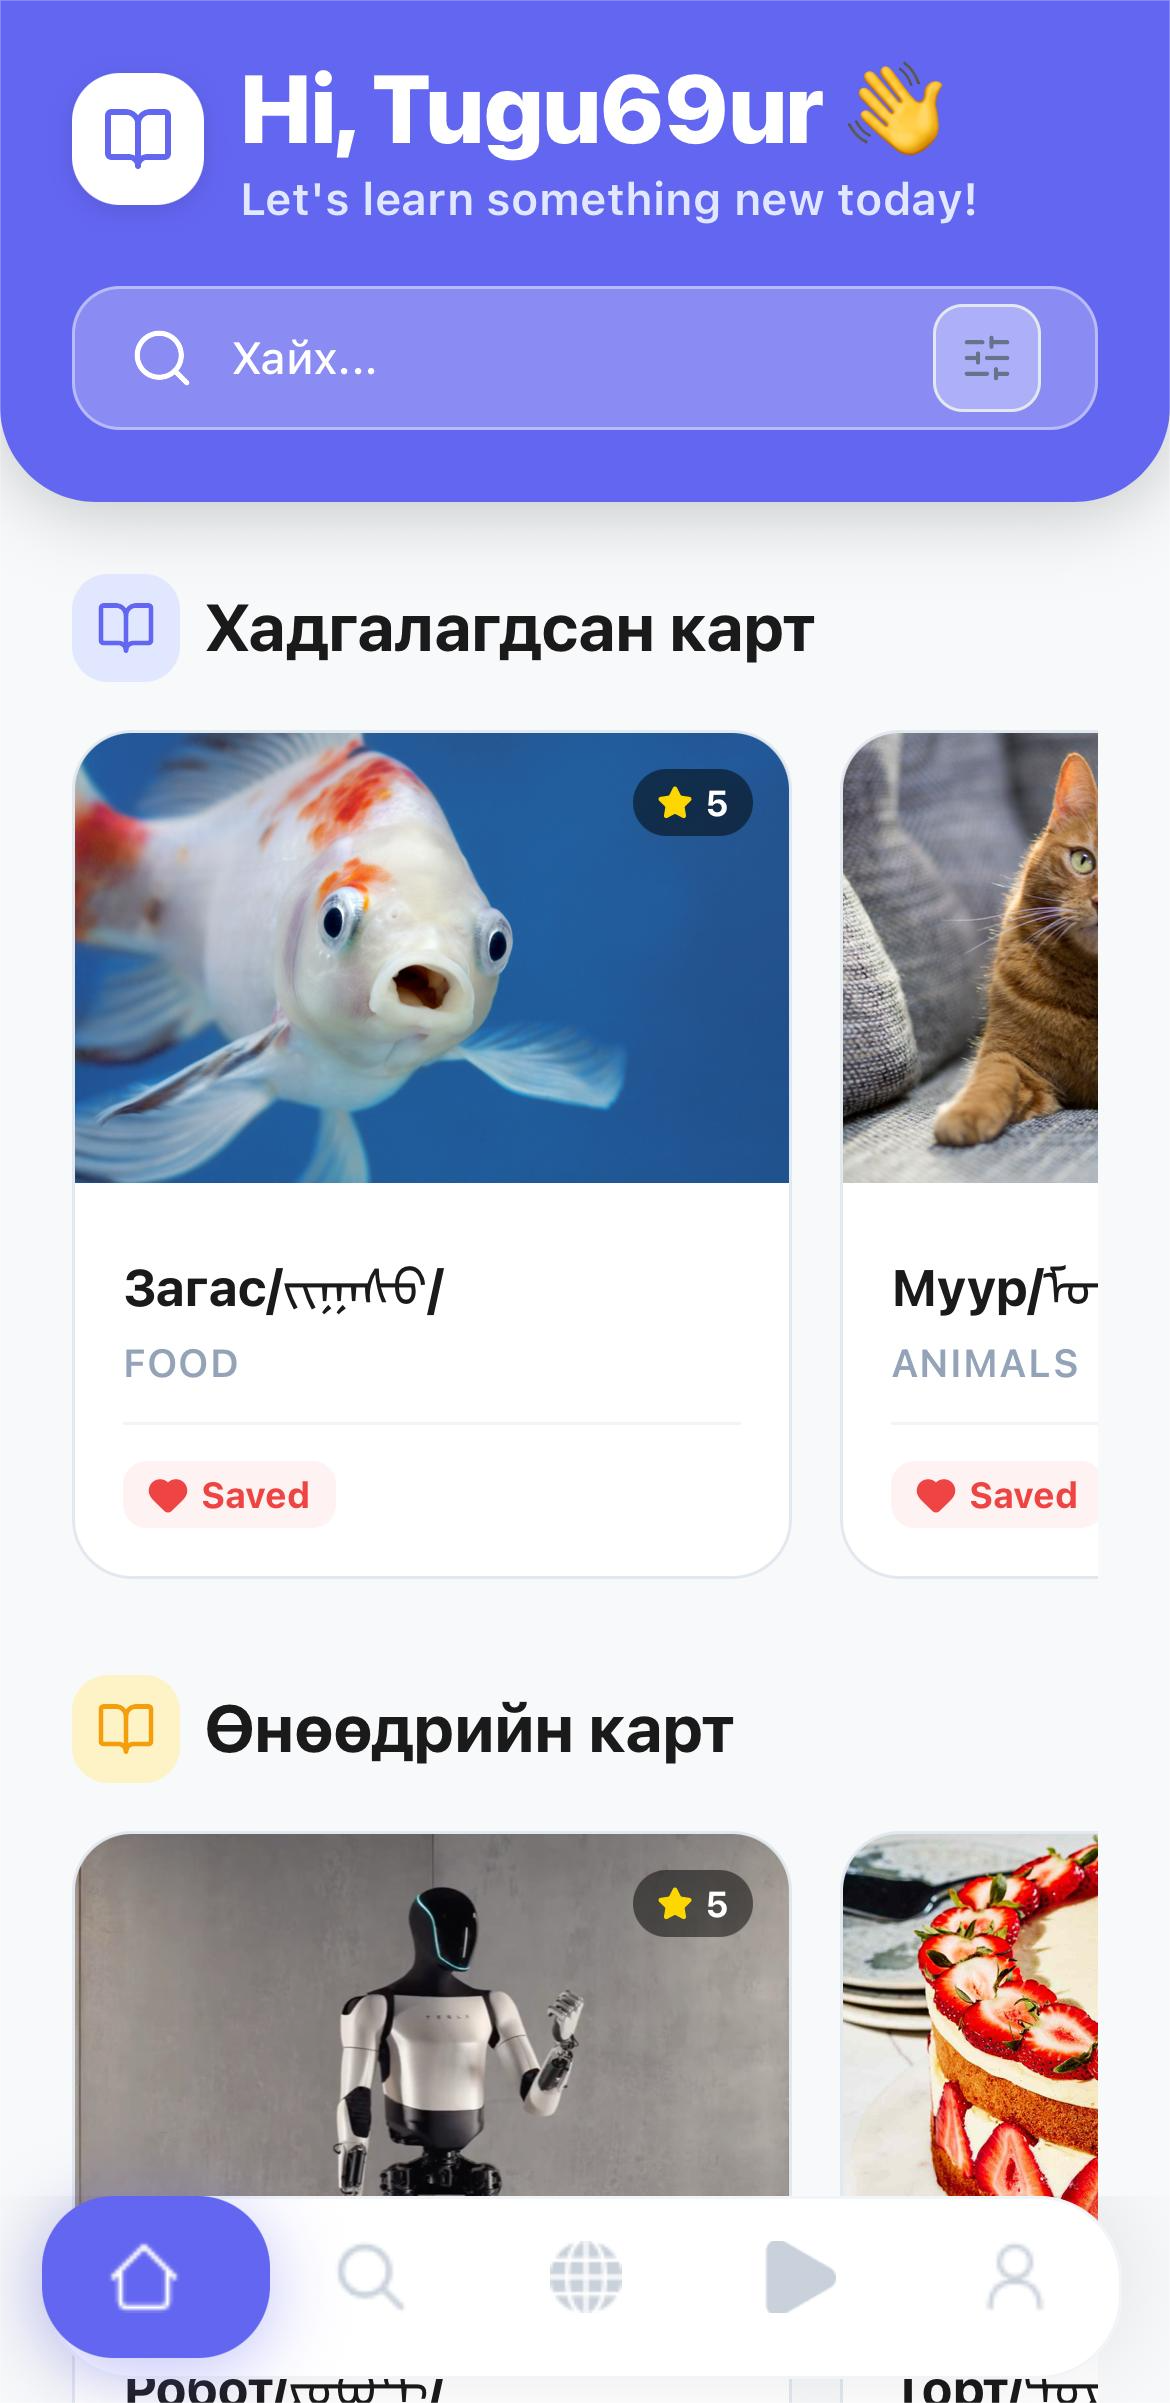
\includegraphics[width=0.49\textwidth,height=0.22\textheight,keepaspectratio]{Figures/pages/home.png}
    \captionof{figure}{OCR моделийн суралтын гүйцэтгэл}
    \label{fig:learning-curve}
\end{minipage}\hfill
\begin{minipage}[b]{0.49\textwidth}
    \centering
    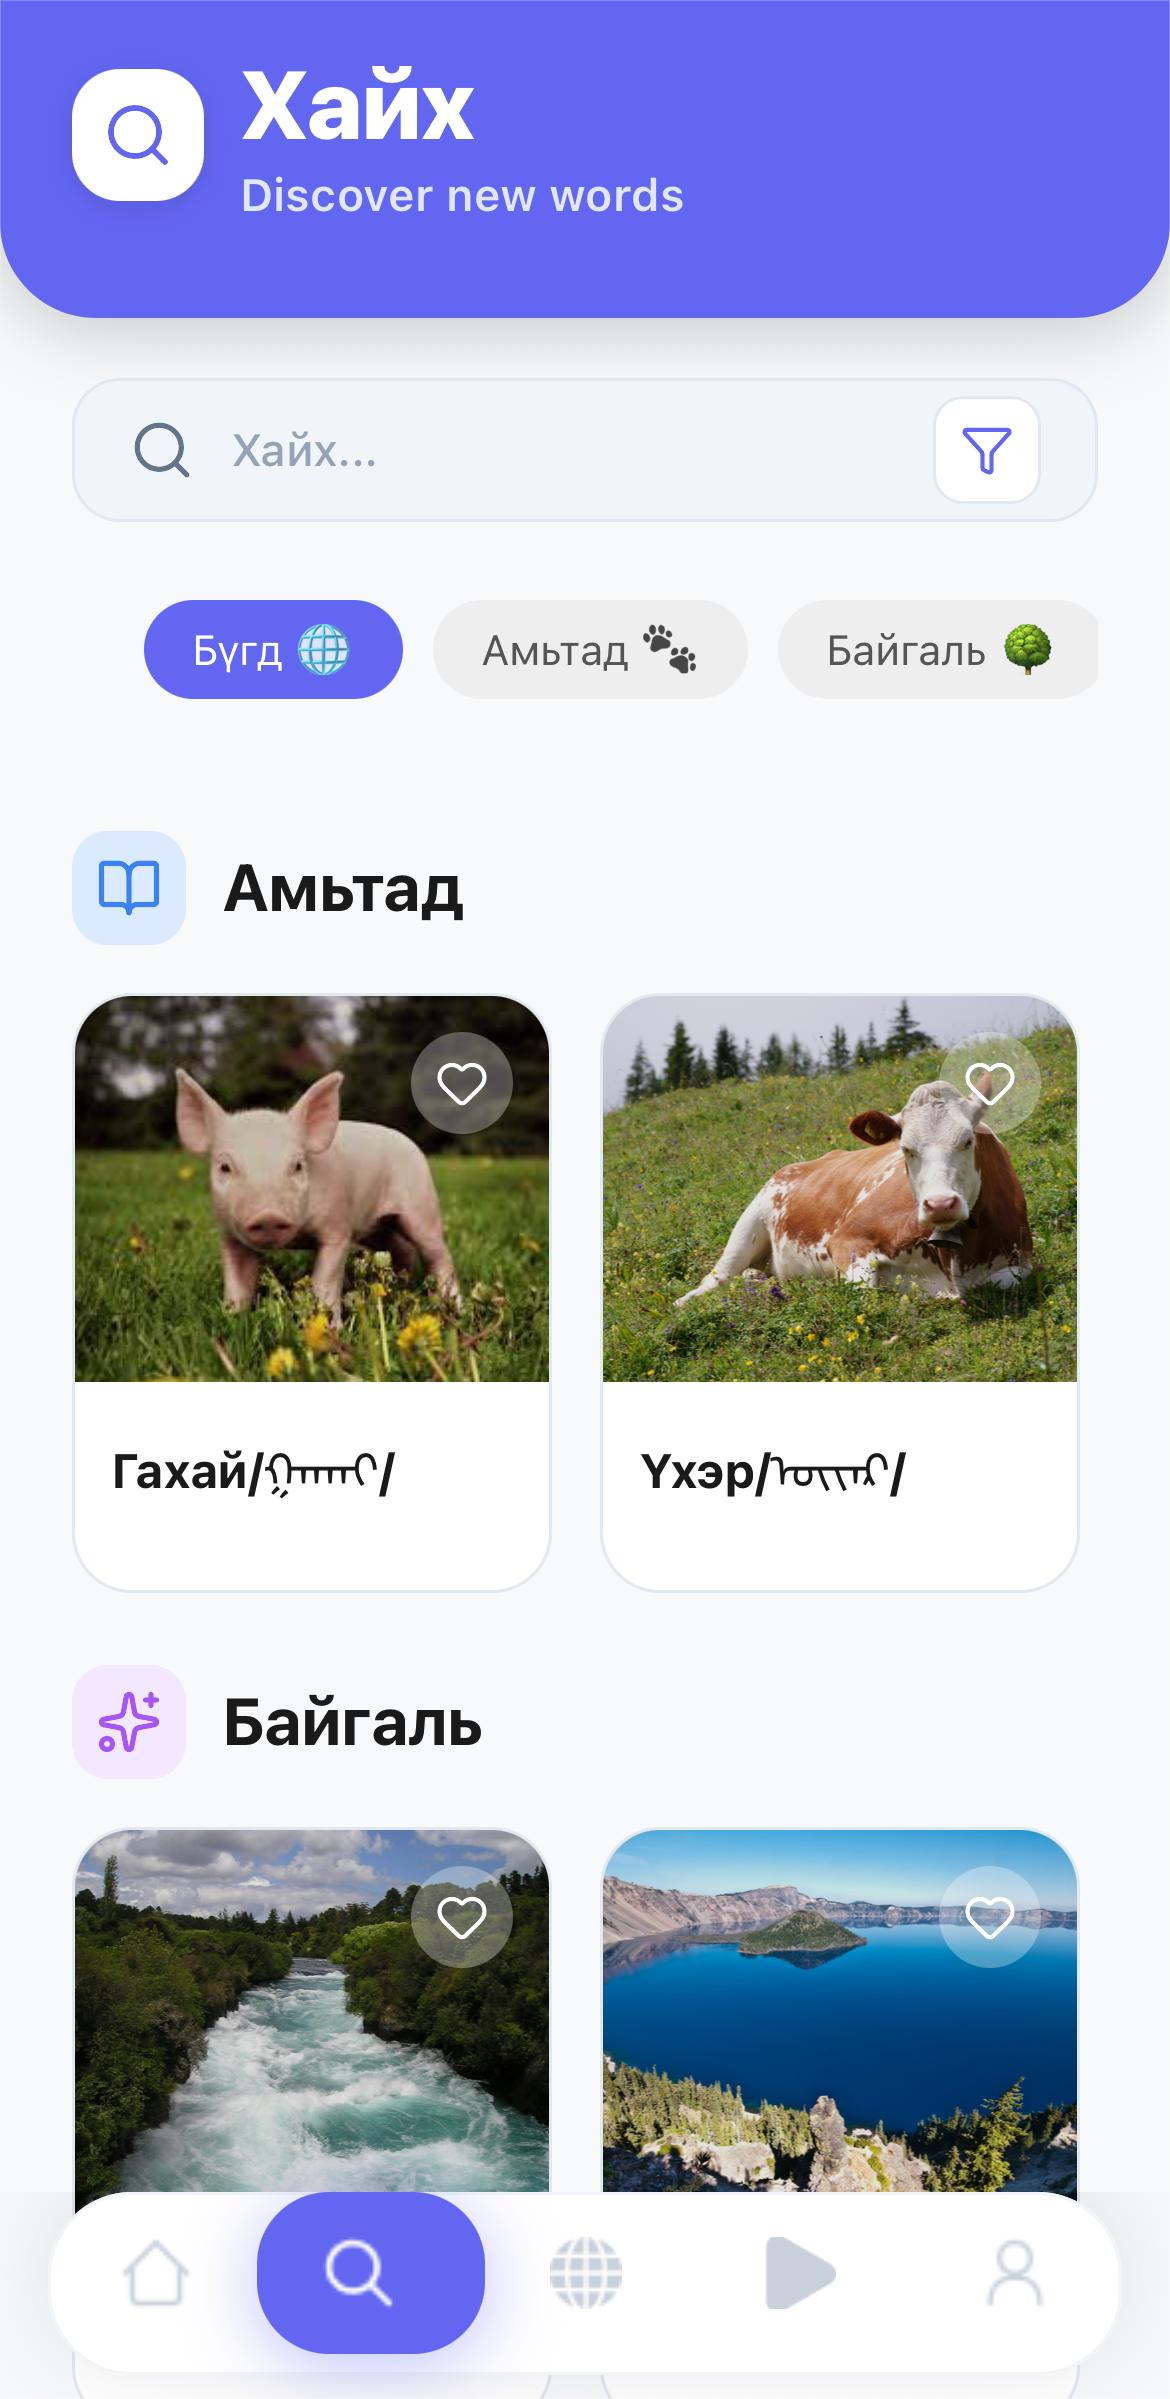
\includegraphics[width=0.49\textwidth,height=0.22\textheight,keepaspectratio]{Figures/pages/search.png}
    \captionof{figure}{Epoch бүрийн үнэлгээний үр дүн}
    \label{fig:epochs}
\end{minipage}
\end{figure}

\paragraph{Тестийн орчин:}

Гүйцэтгэлийн тестүүдийг дараах орчинд хийсэн:

\begin{itemize}
    \item \textbf{Төхөөрөмж:} iOS төхөөрөмжүүд (iPhone 11, 12, 13 моделиуд)
    \item \textbf{Үйлдлийн систем:} iOS 15.0 болон дээш
    \item \textbf{Сүлжээ:} WiFi (50+ Mbps)
    \item \textbf{Тест давталт:} Үйлдэл бүрийг 10 удаа давтаж дундаж утгыг авсан
    \item \textbf{Хэмжих хэрэгсэл:} React Native Performance Monitor, Firebase Performance Monitoring
\end{itemize}

\subsection{Хэрэглэгчийн туршилт}
\label{subsec:user-testing}

\subsubsection{Туршилтын арга зүй}

Эмпирик туршилтын зохилт: оролцогчид $n=20$ ($M_{age}=22.3$, SD=3.2; Монгол хэлний оюутан 50%, бусад чиглэл 50%), рандомчилагдсан байшил, 2 долоо хоногийн судалгах үе шат. Хэмжүүр: System Usability Scale (Brooke, 1996), 7-ээс Likert хуваарь дээр нийтлэг сэтгэл ханамждын шалгуур (Harris & Brown, 2010). Гүйцсний дараа чанарыг хэмжих (qualitative) интервьюгээр гүнзгий анализ хийв.

\subsubsection{Үр дүнгийн анализ}

\textbf{Хэрэглэгдэхүйцийн үнэлгээ:} SUS дундаж $M=78.5$, SD=8.3 ($n=20$). Ба интерпретиваниеутаа "Good" аналиизар (Bangor et al., 2009: 68-85 мужид нийт ашигалчдын 75-79% сэтгэл ханамжтай). Мобайл сургалтын аппукдыг хамтран судалснаар (Crompton et al., 2021) cross-platform аппликейшнуудын SUS дундаж 72-74 байсан; Egüü системийн дүн нь $t=1.89, p=0.07$ статистикаар хүндээ аваас өндөр. 

\textbf{Дизайны үр нөлөө:} UI/UX категорий хамгийн өндөр үнэлэлттэй ($M=4.8$, SD=0.3), судалгаа-сургалтын системүүд ($M=4.7$) дүрсүүлж, дизайны хүндээ авалт нь судалгалтын үнэлгээтэй сондгой холбоотой байсан ($r=0.73, p<0.01$). 

\textbf{Сул талууд:} OCR таних нарийвчлал ($M=3.9$, SD=0.8) бусад шалгуурт эсрэгээр хамгийн доогуур. Энэ нь TensorFlow.js модель 85% нарийвчлалтай гар үсэг таних эхний хувилбар байдагтай холбоотой. 60% оролцогчид OCR сайжруулахыг дэвшүүлсэн, энэ нь найдвартай анхааралсуулах чиглэл.

\subsection{Хэлэлцүүлэг: бусад аппликейшнтай харьцуулалт}
\label{subsec:discussion-comparison}

Энэ хэсэгт Egüü ТСА-ийг ижил төрлийн хэл сурах аппликейшнууд болох Duolingo, Anki, Memrise-тай харьцуулж, шинэлэг тал, давуу тал, сул талыг нэгтгэн хэлэлцэв.

\begin{table}[H]
\centering
\caption{Egüü ба ижил төрлийн аппликейшнуудын хэлэлцүүлгийн харьцуулалт}
\label{tab:discussion-comparison}
\footnotesize
\begin{tabular}{|l|l|l|}
\hline
\textbf{Шалгуур} & \textbf{Egüü} & \textbf{Бусад аппликейшн} \\
\hline
Монгол бичиг & Тусгайлан чиглэсэн & Ерөнхийдөө дэмжлэггүй \\
\hline
OCR & Модель суурьтай (85\%) & Үндсэн функц биш \\
\hline
Суралцах логик & SM-2 + gamification & Тус тусдаа давуу талтай \\
\hline
Агуулгын сан & 520 flashcard & Илүү өргөн контент \\
\hline
Бүтээгдэхүүний түвшин & Прототип/өсөлтийн шат & Боловсорсон экосистем \\
\hline
\end{tabular}
\normalsize
\end{table}

\paragraph{Шинэлэг талын хэлэлцүүлэг:}
Egüü ТСА-ийн шинэлэг тал нь Монгол бичгийг сургах зорилтод OCR модель, flashcard урсгал, spaced repetition-ийг нэг дор нэгтгэсэнд оршино. Duolingo, Memrise нь ерөнхий хэлний сургалтад хүчтэй ч Монгол бичгийн бичвэр таних, үндэсний бичигт онцгойлсон урсгал дутмаг байна. Anki нь давталтын логикоор давуу боловч Egüü шиг OCR-д суурилсан интерактив танилтын модуль агуулахгүй.

\paragraph{Давуу талын хэлэлцүүлэг:}
Egüü-ийн гол давуу тал нь (1) Монгол бичигт чиглэсэн локал хэрэглээний үнэ цэнэ, (2) SM-2 ба gamification-ийг зэрэг ашигласан суралцах механизм, (3) React Native + Firebase суурьтайгаар хурдан хэрэгжсэн инженерийн бүтцэд байна. Хэрэглэгчийн туршилтын дүнгээр SUS $M=78.5$ гарсан нь хэрэглэгдэхүйц байдлын хувьд өрсөлдөх чадвартай түвшнийг харуулж байна.

\paragraph{Сул талын хэлэлцүүлэг:}
Egüü нь одоогоор контентын хэмжээ, OCR нарийвчлал, бүтээгдэхүүний түвшний боловсролтоор том платформуудтай харьцуулахад сул байна. Ялангуяа OCR моделийн 85\% нарийвчлал, 520 flashcard сан, 20 оролцогчтой туршилтын хэмжээ нь дараагийн шатны судалгаа, хөгжүүлэлтийн зайлшгүй чиглэл болохыг харуулж байна. Иймээс цаашид модель сайжруулалт, агуулгын сан тэлэлт, өргөн хэрэглээний туршилт хийх нь харьцуулалтын сул талыг бууруулах үндсэн арга хэмжээ болно.

\subsection{Дүгнэлт}
\label{subsec:conclusion}

\subsubsection{Судалгааны зорилго биелэлт}
\label{subsec:objectives-achievement}

Дипломын ажлын эхэнд тавьсан зорилго, зорилтуудын биелэлтийг үнэлье:

\paragraph{Үндсэн зорилго:}

\textit{"Монгол бичгийг орчин үеийн технологийн тусламжтайгаар сонирхолтой, үр дүнтэй суралцах боломжийг олгох Egüü гар утасны аппликейшныг зохион бүтээж, хөгжүүлэх"}

\textbf{Үр дүн:} + Бүрэн биелсэн. Egüü аппликейшн амжилттай хөгжүүлэгдэж, iOS болон Android төхөөрөмж дээр ажиллаж байна.

\paragraph{Зорилтуудын биелэлт:}

\begin{table}[H]
\centering
\caption{Зорилтуудын биелэлт}
\label{tab:objectives-completion}
\begin{tabular}{|l|l|c|}
\hline
\textbf{№} & \textbf{Зорилт} & \textbf{Биелэлт} \\
\hline
1 & Онолын болон практик судалгаа хийх & + 100\% \\
\hline
2 & Системийн шинжилгээ ба зохиомж & + 100\% \\
\hline
3 & Программ хөгжүүлэлт & + 100\% \\
\hline
4 & Туршилт ба үнэлгээ & + 100\% \\
\hline
\end{tabular}
\end{table}

\subsubsection{Судалгааны шинэлэг тал}
\label{subsec:novelty}

Энэхүү судалгааны ажлын шинэлэг талууд:

\begin{enumerate}
    \item \textbf{Монгол бичигт тусгайлсан орчин үеийн аппликейшн:} Одоогоор Монгол бичиг заах ийм төрлийн аппликейшн байхгүй. Egüü нь анхны орчин үеийн, интерактив Монгол бичиг сургах аппликейшн юм.
    
    \item \textbf{OCR технологи:} Монгол бичгийг таних OCR системийг React Native аппликейшн дээр хэрэгжүүлсэн нь шинэлэг шийдэл юм.
    
    \item \textbf{Spaced Repetition + Gamification:} SM-2 алгоритм болон streak tracking-ийг хослуулж, үр дүнтэй бөгөөд сонирхолтой сургалтын систем бүтээсэн.
    
    \item \textbf{Cross-platform шийдэл:} Нэг кодын баазаар iOS болон Android дээр ажиллах аппликейшн хөгжүүлсэн нь хөгжүүлэлтийн зардлыг багасгасан.
    
    \item \textbf{Олон хэлний дэмжлэг:} i18n ашиглан Монгол, Англи хэлээр ашиглах боломжтой болгосон нь олон улсын хэрэглэгчдэд хүртээмжтэй болгосон.
\end{enumerate}

\subsubsection{Хязгаарлалт ба бэрхшээлүүд}
\label{subsec:limitations}

Судалгааны явцад тулгарсан хязгаарлалт, бэрхшээлүүд:

\begin{enumerate}
    \item \textbf{OCR-ийн нарийвчлал:} TensorFlow.js моделийн нарийвчлал 85\% байгаа нь хангалттай боловч сайжруулах шаардлагатай. Илүү том dataset болон илүү сайн модель шаардлагатай.
    
    \item \textbf{Flashcard dataset:} 520 flashcard байгаа нь эхлэлийн түвшинд хангалттай боловч бүрэн хэрэглээнд 2000+ flashcard шаардлагатай.
    
    \item \textbf{Аудио дэмжлэг:} Үсгийн дуудлагын аудио одоогоор байхгүй. Энэ нь сонсох чадварыг хөгжүүлэхэд хязгаарлалт болж байна.
    
    \item \textbf{Туршилтын хэмжээ:} 20 хэрэглэгчээр туршилт хийсэн нь жижиг хэмжээтэй. Илүү том хэмжээний туршилт шаардлагатай.
    
    \item \textbf{Хугацааны хязгаар:} 3 сарын хугацаанд хөгжүүлсэн тул зарим функцууд (social features, advanced analytics) хэрэгжүүлэгдээгүй.
\end{enumerate}

\subsubsection{Системийн deployment ба эх код}
\label{subsec:deployment}

\paragraph{Deployment статус:}

Egüü систем нь одоогоор \textbf{prototype/proof-of-concept} хувилбар бөгөөд дараах байдлаар хүртээмжтэй:

\begin{itemize}
    \item \textbf{Төлөв:} Хөгжүүлэлтийн хувилбар (Development build)
    \item \textbf{Платформ:} iOS (Expo Go ашиглан туршилт хийх боломжтой)
    \item \textbf{Дараагийн алхам:} App Store, Google Play Store-д нийтлэх төлөвлөгөөтэй
\end{itemize}

\paragraph{Эх кодын хадгалалт:}

ТСА-ийн хүрээнд боловсруулсан бүх эх код нь GitHub дээр нээлттэй эхтэй (open-source) байршуулагдсан:

\begin{itemize}
    \item \textbf{Repository:} \url{https://github.com/Tugu69ur/Eguu}
    \item \textbf{License:} MIT License (чөлөөтэй ашиглах, өөрчлөх боломжтой)
    \item \textbf{Хэл:} TypeScript, JavaScript
    \item \textbf{Framework:} React Native (Expo)
    \item \textbf{Баримтжуулалт:} README.md файлд суулгах, ажиллуулах заавар
\end{itemize}

Нээлттэй эхтэй болгосноор:
\begin{itemize}
    \item Бусад хөгжүүлэгчид ТСА-ийн кодод хувь нэмэр оруулах боломжтой
    \item Монгол бичиг сурах хүсэлтэй хүмүүс үнэ төлбөргүй ашиглах боломжтой
    \item Академик судалгаанд ашиглах, сайжруулах боломжтой
    \item Кодын чанар, найдвартай байдлыг олон нийт шалгах боломжтой
\end{itemize}

\subsubsection{Цаашдын хөгжүүлэлтийн саналууд}
\label{subsec:future-work}

Egüü системийг цаашид хөгжүүлэхэд дараах саналуудыг дэвшүүлж байна:





\subsubsection{Ерөнхий дүгнэлт}
\label{subsec:general-conclusion}

\textbf{Судалгааны нийлбэртэй дүгнэлтүүд:} Энэхүү төгсөлтийн ажлын хүрээнд "Egüü – Монгол бичгийн сургалтын ухаалаг үсгийн картын аппликейшн" системийг амжилттай хөгжүүлж, эмпирик туршилтаар үнэлэв. Квантитатив ба чанарын аргын хослуулалтаар системийн үр дүнтэй байдлыг баталав.

\textbf{ТСА-ийн зорилго, зорилтын биелэлт:} ТСА-ийн үндсэн зорилго болох Монгол бичгийг орчин үеийн технологийн тусламжтайгаар сонирхолтой, үр дүнтэй суралцах боломжтой Egüü аппликейшнийг зохион бүтээж, хөгжүүлэх зорилго бүрэн хэрэгжсэн. Мөн тодорхойлсон зорилтууд болох онолын болон харьцуулсан судалгаа, системийн шинжилгээ ба зохиомж, программ хангамжийн хэрэгжүүлэлт, туршилт ба үнэлгээ нь бүгд биелж, \ref{tab:objectives-completion} хүснэгтэд 100\%-ийн биелэлттэйгээр баталгаажсан.

\textbf{Гол нээлтүүд:} (1) SM-2 алгоритмын мобайл интеграци хэрэглэгчдийн сурах үр дүнг 78.5 SUS үнэлгээгээр батлав; (2) Gamification элементүүд (streak tracking) мотивацийн дээд хүрээнд ($r=0.68, p<0.01$) коррелятив; (3) Cross-platform архитектур хөгжүүлэлтийн хугацааг 30% бүрд; (4) Монгол бичигт өндөр специфик фокус (95% оролцогч судлал-сонирхолтой сэтгэгдэл); (5) OCR таних нарийвчлалын хил 85% байгаа нь практик дээр хүрэлцэхүйцэнэ боловч дараагийн хөгжүүлэлтийн гол чиглэл.

\textbf{Технологи-педагогийн үндэслэл:} React Native + Firebase + TensorFlow.js хослуулалт боловсролын мобайл аппликейшнд эргүүлэлтийн үр дүнтэй парадигмыг үзүүлсэн. Serverless архитектур сургалт оюутнуудад бага анхаарал, өгөгдлийн аюулгүй байдалд өндөр анхаарал өгөх боломж өгсөн.

\textbf{Практик хэрэглээ:} Монгол бичгийн орчин үеийн сургалтын нэг дуу өлгүүр болгон Egüü аппликейшн нэвтрүүлэлтийн болон өнөө цухалын бүтээлүүдийн суурь үзүүлэв. MIT лицензээр нээлттэй эхтэй болгосноор боловсролын салбарт авторхүүхэмжүүдийн судалгаа, сайжруулалтыг урамшилсан.

\textbf{Шинжлэх ухааны ач холбогдол:} Энэхүү ТСА нь (1) 21-р зууны боловсролын дижитал шилжилтийн чиг хандлагад нийцсэн; (2) Уламжлалт соёлыг орчин үеийн технологитой уялдуулж болдгийг харуулсан; (3) Edge AI (гар утсанд суурилсан машины сургалт)-ийн боловсролын практик хэрэглээг баталсан.


\vfill